\documentclass[14pt]{mmcs_article}
\usepackage[russian]{babel}
\usepackage{amsmath, amsthm, amsfonts, amssymb}

\graphicspath{{images/}}%путь к рисункам

\begin{document}

% Титульные листы
% раскомментировать требуемое
%%см. РЕКОМЕНДАЦИИ ПО ОФОРМЛЕНИЮ
%И ПРЕДСТАВЛЕНИЮ КУРСОВЫХ И ВЫПУСКНЫХ %КВАЛИФИКАЦИОННЫХ РАБОТ СТУДЕНТОВ ИНСТИТУТА %МАТЕМАТИКИ, МЕХАНИКИ И КОМПЬЮТЕРНЫХ НАУК


% ----------------------------------
% Внимание!
% Изменяйте только строки, перед которыми стоят знаки комментариев
% ----------------------------------

\thispagestyle{empty}
\begin{singlespacing}
\begin{center}

МИНОБРНАУКИ РОССИИ\\ [12pt]
Федеральное государственное автономное образовательное\\
учреждение высшего образования\\
<<Южный федеральный университет>>

\vspace{\baselineskip}
Институт математики, механики\\
и компьютерных наук им.~И.\,И.~Воровича

\vspace{\baselineskip}
% Название выпускающей кафедры
Кафедра алгебры и дискретной математики

\vfill
% Фамилия Имя Отчество студента
\textbf{Иванов Сергей Иванович}

\vspace{\baselineskip}
%%НАЗВАНИЕ РАБОТЫ должно полностью соответствовать распоряжению по Институту (для курсовых работ).
{\bf НАЗВАНИЕ РАБОТЫ, \\
РАЗБИТОЕ ПРИ НЕОБХОДИМОСТИ \\
НА НЕСКОЛЬКО СТРОК }

\vspace{15mm}
КУРСОВАЯ РАБОТА\\
по направлению подготовки\\
% указать направление обучения (раскомментируйте нужную строчку)
01.03.02~-- Прикладная математика и информатика
% 01.03.01~-- Математика
% 01.03.03~-- Механика и математическое моделирование 	
% 02.03.02~-- Фундаментальная информатика и информационные технологии


\vspace{10mm}
\textbf{Научный руководитель~--}\\
% указать данные о руководителе
% должность, степень, звание Фамилия Имя Отчество
проф., д.\,ф.-м.\,н. Сергеев Петр Сергеевич

\vspace{20mm}

\noindent
\begin{flushleft}
$\overline{\textrm{оценка (рейтинг)}}$\qquad	$\overline{\textrm{подпись руководителя\vphantom{й}}}$

\end{flushleft}


\vfill
% год!
Ростов-на-Дону -- 2020

\end{center}

\singlespacing
\end{singlespacing}  % для курсовой
%см. РЕКОМЕНДАЦИИ ПО ОФОРМЛЕНИЮ
%И ПРЕДСТАВЛЕНИЮ КУРСОВЫХ И ВЫПУСКНЫХ %КВАЛИФИКАЦИОННЫХ РАБОТ СТУДЕНТОВ ИНСТИТУТА %МАТЕМАТИКИ, МЕХАНИКИ И КОМПЬЮТЕРНЫХ НАУК


% ----------------------------------
% Внимание!
% Изменяйте только строки, перед которыми стоят знаки комментариев
% ----------------------------------

\thispagestyle{empty}
\begin{singlespacing}
\begin{center}

МИНОБРНАУКИ РОССИИ\\ [12pt]
Федеральное государственное автономное образовательное\\
учреждение высшего образования\\
<<Южный федеральный университет>>

\vspace{\baselineskip}
Институт математики, механики\\
и компьютерных наук им.~И.\,И.~Воровича

\vspace{\baselineskip}
% Название выпускающей кафедры
Кафедра информатики и вычислительного эксперимента

\vfill
% Фамилия Имя Отчество студента
\textbf{Волнобой Ирина Леонидовна}

\vspace{\baselineskip}
%НАЗВАНИЕ РАБОТЫ должно полностью соответствовать
% приказу по ЮФУ (для выпускных квалификационных работ)
{\bf РАЗРАБОТКА КОМПОНЕНТОВ ПРИЛОЖЕНИЯ \\
ДЛЯ АНАЛИЗА ОНЛАЙН-ПРОФИЛЯ \\
ЖИВОТНОГО ИЗ ПРИЮТА }


\vspace{15mm}
ВЫПУСКНАЯ КВАЛИФИКАЦИОННАЯ РАБОТА\\
по направлению подготовки\\
% Направление обучения
% раскомментируйте нужную строчку
02.03.02~-- Фундаментальная информатика и информационные технологии
% 01.03.01~-- Математика
% 01.03.02~-- Прикладная математика и информатика
% 01.03.03~-- Механика и математическое моделирование 	


\vspace{10mm}
\textbf{Научный руководитель~--}\\
% указать данные о руководителе
% должность, степень, звание Фамилия Имя Отчество 
доцент., к.\,ф.-м.\,н. Абрамян Анна Владимировна

\vspace{15mm}

\noindent
% указать Фамилию и инициалы 
% заведующего выпускающей кафедры
\begin{flushleft}
Допущено к защите:\\
заведующий кафедрой \underline{\hspace*{65mm}} Михалкович С.\,С.
\end{flushleft}




\vfill
% год!
Ростов-на-Дону -- 2021

\end{center}

\singlespacing
\end{singlespacing} % для работы бакалавра
%%см. РЕКОМЕНДАЦИИ ПО ОФОРМЛЕНИЮ
%И ПРЕДСТАВЛЕНИЮ КУРСОВЫХ И ВЫПУСКНЫХ %КВАЛИФИКАЦИОННЫХ РАБОТ СТУДЕНТОВ ИНСТИТУТА %МАТЕМАТИКИ, МЕХАНИКИ И КОМПЬЮТЕРНЫХ НАУК


% ----------------------------------
% Внимание!
% Изменяйте только строки, перед которыми стоят знаки комментариев
% ----------------------------------

\thispagestyle{empty}
\begin{singlespacing} 
\begin{center}

МИНОБРНАУКИ РОССИИ\\ [12pt]
Федеральное государственное автономное образовательное\\
учреждение высшего образования\\
<<Южный федеральный университет>>

\vspace{\baselineskip}
Институт математики, механики\\
и компьютерных наук им.~И.\,И.~Воровича


\vfill
% Фамилия Имя Отчество студента
\textbf{Иванов Сергей Иванович}

\vspace{15mm}
%НАЗВАНИЕ РАБОТЫ должно полностью соответствовать 
% приказу по ЮФУ (для выпускных квалификационных работ)
{\bf НАЗВАНИЕ РАБОТЫ, \\
РАЗБИТОЕ ПРИ НЕОБХОДИМОСТИ \\
НА НЕСКОЛЬКО СТРОК }

\vspace{15mm}
ВЫПУСКНАЯ КВАЛИФИКАЦИОННАЯ РАБОТА\\
по направлению подготовки\\
% Направление обучения 
01.04.02~-- Прикладная математика и информатика,\\
направленность программы\\
<<Математическое и программное обеспечение вычислительных машин>>

\vspace{10mm}
\textbf{Научный руководитель~--}\\
% указать данные о руководителе
% должность, степень, звание Фамилия Имя Отчество
проф., д.\,ф.-м.\,н. Сергеев Петр Сергеевич

\vspace{7mm}
\textbf{Рецензент~--}\\
% указать данные о рецензенте
% должность, степень, звание Фамилия Имя Отчество
доц., к.\,т.\,н. Петров Иван Петрович


\vspace{15mm}

\noindent
% указать Фамилию и инициалы руководителя
% образовательной программы
\begin{flushleft}
Допущено к защите:\\
руководитель \\
образовательной программы \underline{\hspace*{65mm}} Федоров Ф.\,Ф.
\end{flushleft}




\vfill
% год!
Ростов-на-Дону -- 2020

\end{center} 

\singlespacing
\end{singlespacing}% для работы магистра

\renewcommand{\contentsname}{Оглавление}

\tableofcontents

%=======================
\newpage
\addcontentsline{toc}{section}{Постановка задачи}

\section*{Постановка задачи}


В постановке задачи коротко (по пунктам) указывается, что необходимо сделать в рамках работы. Раздел <<Постановка задачи>> должен соответствовать заданию на курсовую или выпускную квалификационную работу, подписанному научным руководителем.


%=======================
\newpage
\addcontentsline{toc}{section}{Введение}
\section*{Введение}

Машинное обучение является одним из подразделов искусственного интеллекта. Оно нашло применение во многих сферах жизни: маркетинге, бизнесе, медицине, в банковской сфере, в различных научных исследованиях. Машинное обучение помогает в решении каких-либо вопросов, помогает принять решение, что нужно улучшить, чтобы увеличить или уменьшить какие-либо показатели и достигнуть цели. 

Например, в данной работе требуется на основе данных о питомцах предсказать, с какой скоростью животное будет принято в семью, а также какие признаки влияют на принятие решения в большей степени. Данная задача предложена к решению малайзийским сайтом petfinder.my. Сама задача, а также все необходимые данные представлены на ресурсе Kaggle [1]. Скорость в данной задаче является категориальной переменной, поэтому необходимо решить задачу классификации. Задача классификации является разновидностью задачи обучения с учителем и решается с помощью методов машинного обучения. 

Для решения данной задачи необходимо проанализировать исходные данные, выбрать наиболее подходящие для задачи методы обработки, применить различные алгоритмы машинного обучения, подобрать параметры, а также сравнить их качество и выбрать наиболее подходящий алгоритм, который показывает наилучшее качество на выбранной метрике.

В данной работе использовался язык программирования Python версии 3.8.2, библиотеки для визуализации matplotlib, seaborn, graphviz, библиотеки для обработки и анализа данных numpy и pandas, а также бибилотеки предоставляющие функционал для предварительной обработки данных и тренировки алгоритмов машинного обучения sklearn, XGBoost, LightGBM. В качестве инструмента для разработки использовался JupyterNotebook.

В качестве предварительной обработки данных использовались следующие методы: 
\begin{itemize}
	\item пропуски в данных заменены выборочным значением
	\item выбросы заменены выборочным значением или введена новая переменная, оценивающая исходную
	\item созданы новые признаки на основе имеющихся
	\item извлечены и обработаны признаки из данных, полученных от Google’s Natural Language API и от Google’s Vision API
	\item применены методы кодирования категориальных переменных: прямое кодирование, One Hot Encoding и Label Encoding
	\item данные приведены к одной шкале с использованием StandardScaler из sklearn
\end{itemize}

Создатели задачи рекомендуют к использованию метрику Quadratic Weighted Kappa, поэтому именно она используется для оценки качества моделей.

Для предсказания класса принятия на основе признаков были использованы алгоритмы логистической регрессии, дерева решений, случайного леса, а также три алгоритма градиентного бустинга из библиотек sklearn, XGBoost и LightGBM. Все модели и способы обработки были оценены и выбран наиболее оптимальный для данной задачи.

Также был использован алгоритм логистической регрессии с алгоритмом оптимизации стохастического градиентного спуска для предсказания целевой переменной на основе только текстовых признаков (описаний животных). Для этого описания животных были предварительно обработаны. Выполнена токенизация, нормализация, стемминг и лемматизация, векторизация методами Bags of Words и TF-IDF. Выполнен анализ эффективности модели на основе данных методов обработки текстов.

Настройка гиперпараметров моделей происходила по сетке с использованием GridSearchCV и RandomizedSearchCV из библиотеки sklearn.




%=======================
\newpage
\addcontentsline{toc}{section}{Обзор}
\section*{Обзор}

%=======================
\newpage
\section{Анализ исходных данных и их предварительная обработка}

\subsection{Описание поставленной задачи и исходных данных}

В данной работе использовались данные представленные на ресурсе Kaggle.  Это два основных датасета, представленных в формате csv:

\begin{itemize}
	\item train.csv --- содержит данные для тренировки модели размерностью 14993 записи на 25 столбцов.
	\item test.csv --- содержит данные для тестирования размерностью 3972 записи на 24 столбца. Данный датасет предназначен для тестирования модели на ресурсе Kaggle.
\end{itemize}

В train.csv на один столбец больше, чем в test.csv, так как тренировочный датасет содержит столбец AdoptionSpeed, который необходимо предсказать в тестовой выборке.

Так же имеется 3 csv файла, являющиеся словарями:

\begin{itemize}
	\item breed\_labels.csv --- словарь пород
	\item color\_labels.csv --- словарь окрасов шерсти
	\item state\_labels.csv --- словарь штатов
\end{itemize}

В словарях содержатся 2 колонки: id и расшифровка. Эти словари необходимы для лучшего понимания данных, так как в тренировочном и тестовом датасетах в колонках содержатся именно id пород, окрасов и штатов, а сами названия находятся в словарях.

Ещё имеются папка, содержащая метаданные, полученные с помощью Google’s Vision API с изображений, и папка, содержащая анализ тональности описаний, представленных в виде текста, который был получен с использованием Google’s Natural Language API. Эти данные представлены в формате PetID.json.

Вся информация, представленная в датасетах была взята создателями соревнования Kaggle с малайзийского сайта petfinder.my (рис. \ref{analyse:petfinder}). Это ресурс, главная задача которого состоит в том, чтоб найти новый дом животным. Анкеты животных на сайт выкладывают либо приюты, либо отдельные люди, которые нашли животное на улице. Несмотря на то, что на самом сайте представлены профили различных видов животных (попугаев, кошек, собак, хомячков, кроликов и так далее), в датасетах содержится информация только о профилях кошек и собак. На этом сайте люди имеют возможность отдать животное в хорошие руки бесплатно или же за определенную плату. Для этого создаётся профиль животного и добавляется туда информация о животном: фотография, кличка, возраст, пол, описание и другое.

\begin{figure}[H]
	\centering
	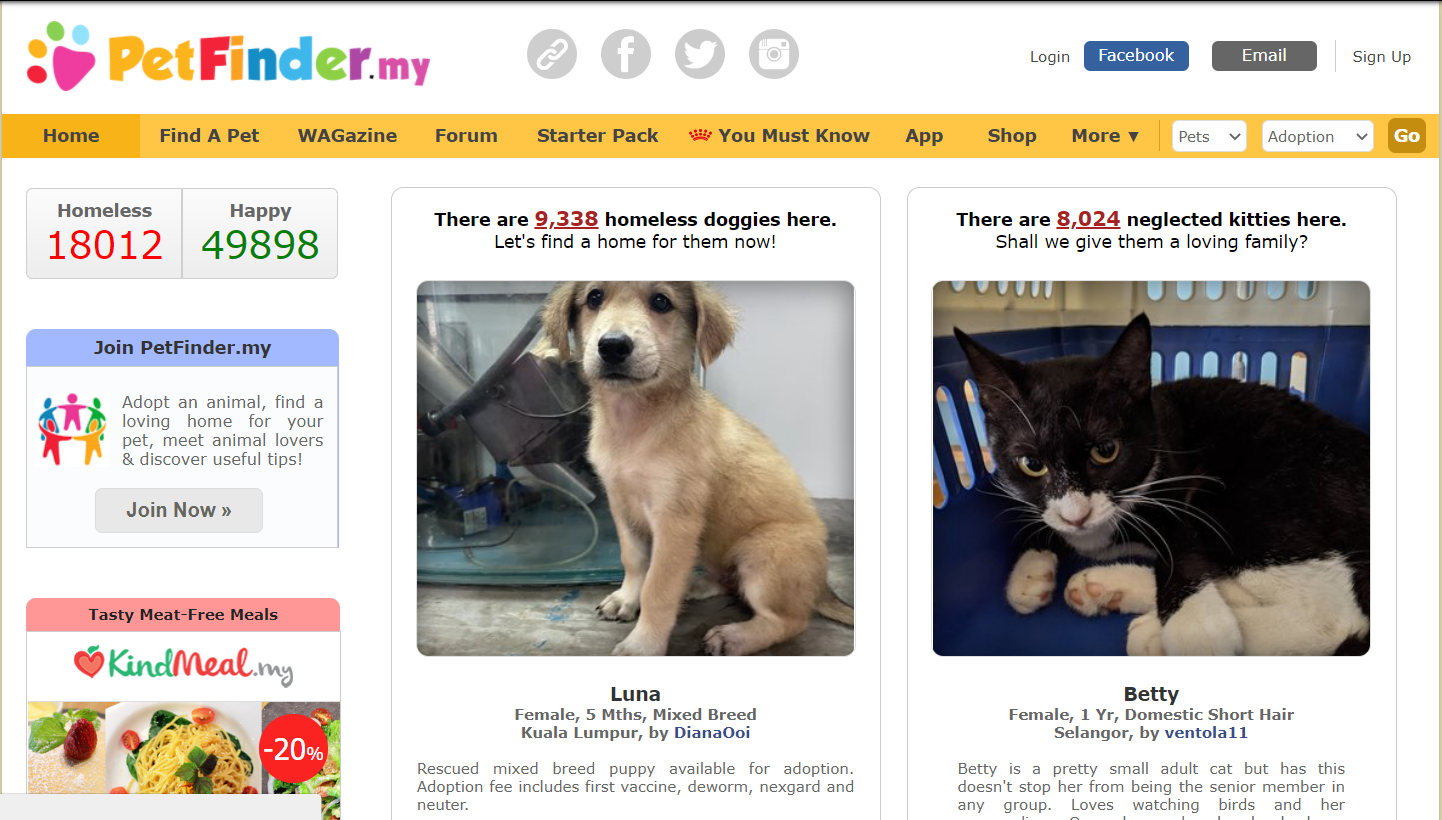
\includegraphics[scale=0.4]{petfinder.png}
	\caption{Скриншот сайта petfinder.my}\label{analyse:petfinder}
\end{figure}


\subsection{Описание признаков}

Всего в датасете присутствует 24 признака. Посмотрим на матрицу корреляции (рис. \ref{analyse:corr}). Наибольший коэффициент корреляции имеют переменные Dewormed и Vaccinated --- 0,72. Но этот коэффициент недостаточно высок для того, чтобы утверждать, что данные переменные линейно зависимы. Поэтому нельзя выбрасывать из рассмотрения ни одну из них. Остальные переменные не коррелируют между собой.

\begin{figure}[H]
	\centering
	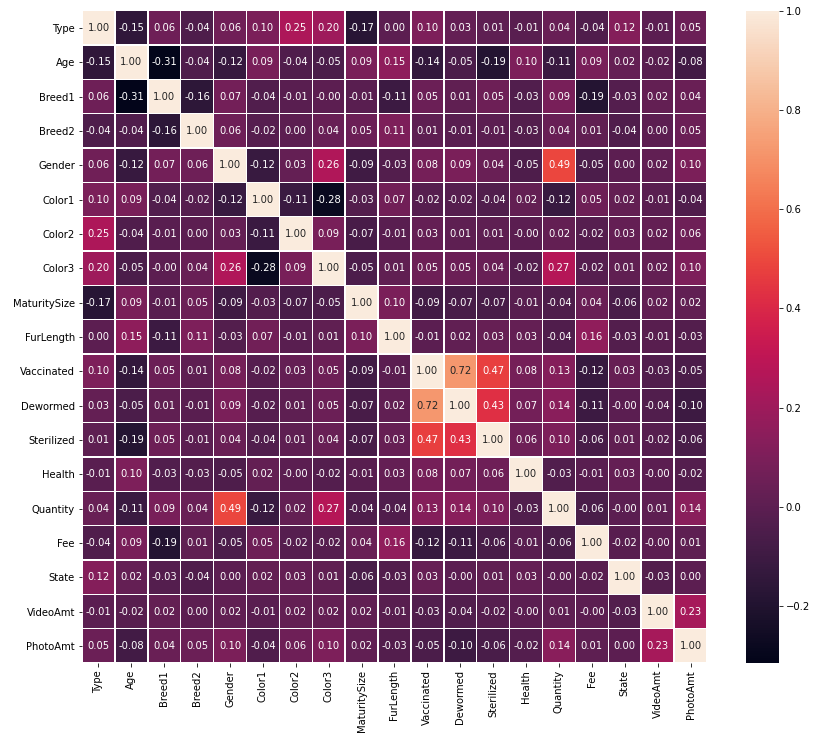
\includegraphics[scale=0.55]{corr.png}
	\caption{Матрица корреляции переменных}\label{analyse:corr}
\end{figure}

Рассмотрим более подробно каждый признак.

PetID --- это уникальный идентификатор питомца. Так как каждый питомец имеет свой идентификатор, то не имеет смысла использовать данный признак для обучения модели.

Type --- тип животного. Это категориальная переменная, принимающая два значения: кошка или собака. Количество собак составляет 8132 особи, а кошек — 6861 (рис. \ref{analyse:type}).

\begin{figure}[H]
	\centering
	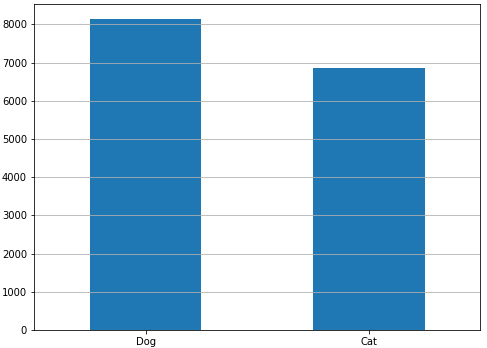
\includegraphics[scale=1.2]{type.png}
	\caption{Распределение кошек и собак в тренировочной выборке}\label{analyse:type}
\end{figure}

Name --- имя питомца. На рисунке \ref{analyse:names} изображены наиболее популярные клички среди кошек и собак. Можно заметить, что большинство людей не придумывали животным имена, а просто называли их “Kitten”, “Puppy” или “No name”. Также была часть животных, имена которых состояли из 1, 2 или 3 символов и не имели смысла. Например, “BB”, “C7C”, “Z4”. 

\begin{figure}[H]
	\centering
	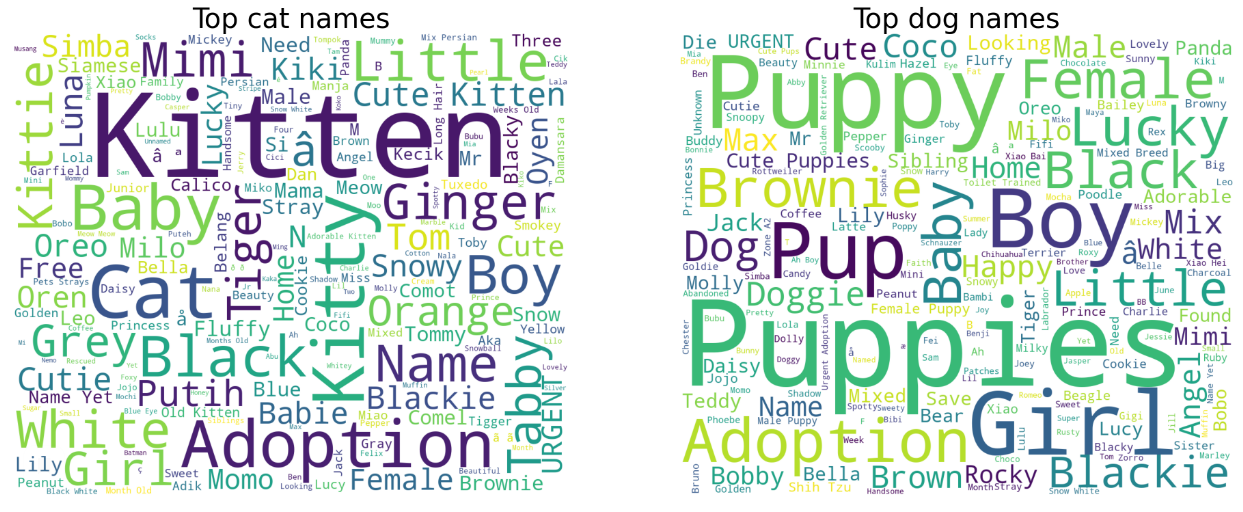
\includegraphics[scale=0.5]{names.png}
	\caption{Наиболее распространённые имена среди кошек и собак}\label{analyse:names}
\end{figure}

Age --- возраст питомца в месяцах.

Breed1 и Breed2 --- переменные, содержащие идентификатор породы, который ссылается на словарь пород breed\_labels.csv. Если питомец чистокровной породы, то в Breed 2 стоит идентификатор 0.

Gender --- категориальная переменная, содержащая пол питомца. Может принимать 3 значения: male, female и mixed. Mixed ставится в том случае, когда в профиле питомцев больше одного. Наибольшее число питомцев имеет мужской пол, наименьшее — смешанный (рис. \ref{analyse:gender})

\begin{figure}[H]
	\centering
	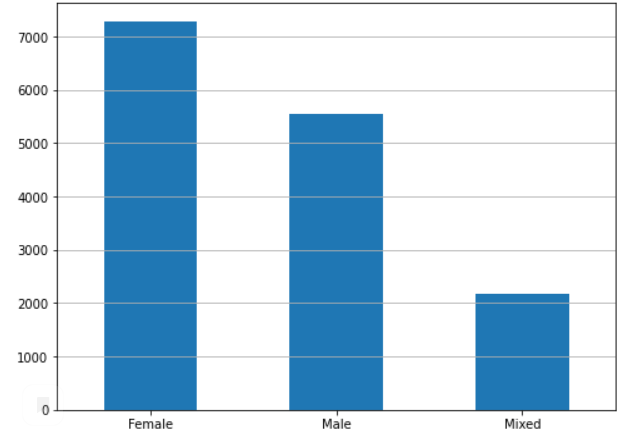
\includegraphics[scale=0.8]{gender.png}
	\caption{Распределение питомцев по полу в train.csv}\label{analyse:gender}
\end{figure}

Переменные Color1, Color2 и Color3 содержат идентификаторы окраса, расшифровка которых находится в файле color\_labels.csv. Если питомец имеет всего один цвет, то в переменных Color2 и Color3 стоит значение 0. Наиболее часто встречаются питомцы коричневого, черно-коричневого и черно-белого цветов (рис. \ref{analyse:color}).

\begin{figure}[H]
	\centering
	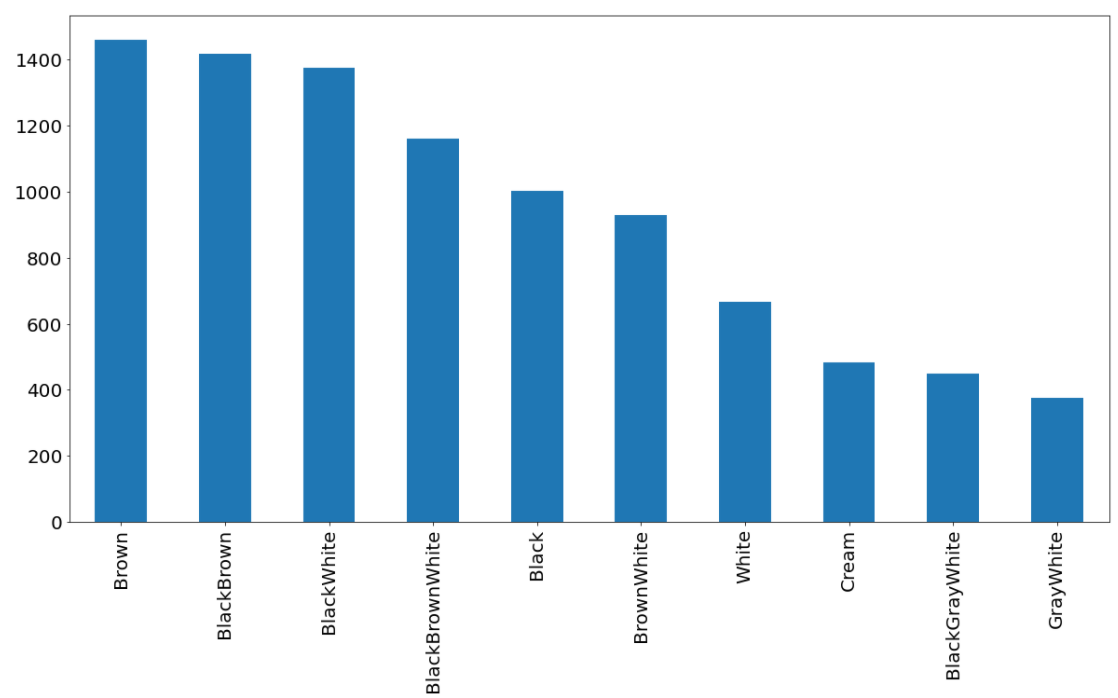
\includegraphics[scale=0.5]{color.png}
	\caption{Наиболее распространнёные комбинации окрасов}\label{analyse:color}
\end{figure}

MaturitySize и FurLength --- категориальные переменные, обозначающие размер в зрелом возрасте и длину шерсти соответственно. MaturitySize принимает 4 значения: ``small'', ``medium'', ``large'' и ``extra large'', а FurLength принимает 3 значения: ``short'', ``medium'', ``long''. Наиболее распространенный размер животного в зрелом возрасте --- средний, а наиболее популярная длина шерсти --- короткая (рис. \ref{analyse:sizelength}).

\begin{figure}[H]
	\centering
	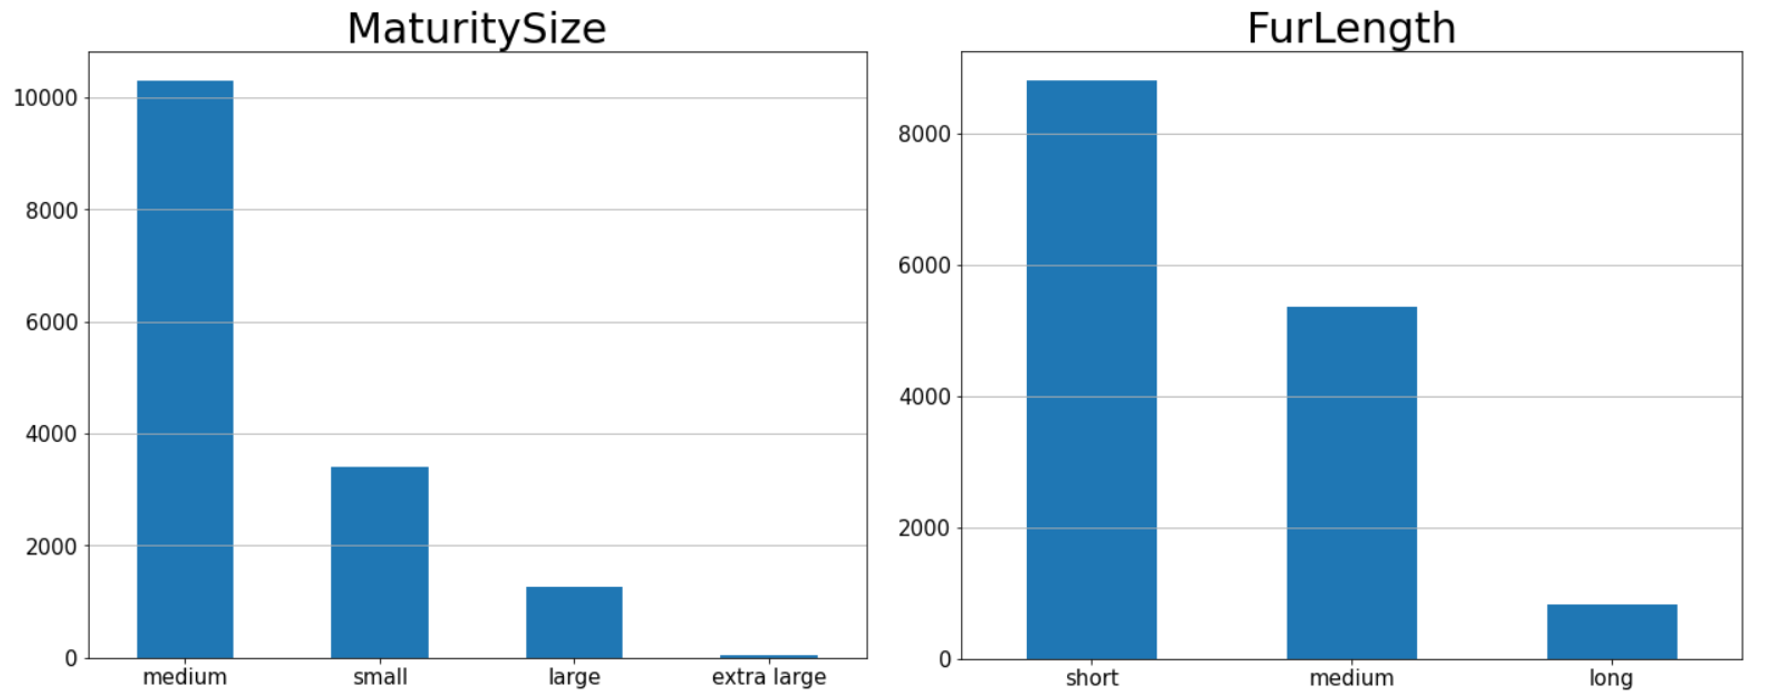
\includegraphics[scale=0.4]{sizelength.png}
	\caption{Наиболее распространнёные комбинации окрасов}\label{analyse:sizelength}
\end{figure}

Также есть 4 категориальных признака, относящихся к здоровью питомца: 

\begin{itemize}
	\item Vaccinated (вакцинировано)
	\item Dewormed (избавлено от гельминтов)
	\item Sterilized (кастрировано)
	\item Health (общее состояние здоровья)
\end{itemize}

Vaccinated, Dewormed и Sterilized принимают 3 значения: ``да'', ``нет'' и ``неизвестно''. Переменная Health также принимает 3 значения: ``Healthy'', ``Minor Injury'', ``Serious Injury''. Большинство животных здоровы, и лишь небольшая часть имеет травмы (рис. \ref{analyse:health}).

\begin{figure}[H]
	\centering
	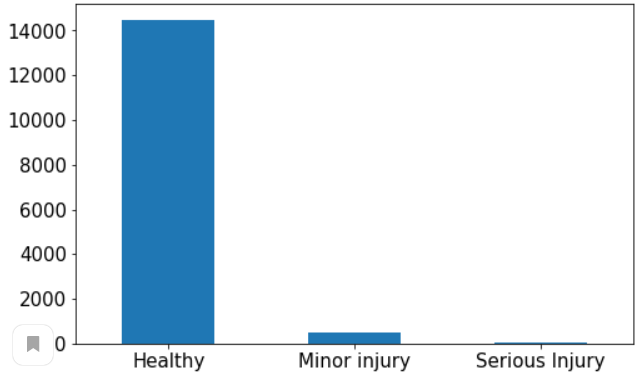
\includegraphics[scale=0.9]{health.png}
	\caption{Состояние здоровья питомцев}\label{analyse:health}
\end{figure}

Quantity --- количество животных в одном профиле. Наибольшее число профилей (11565) содержит одно животное, но также есть записи, где имеется и по 5, и по 10, и даже по 20 животных (рис. \ref{analyse:count}). 

\begin{figure}[H]
	\centering
	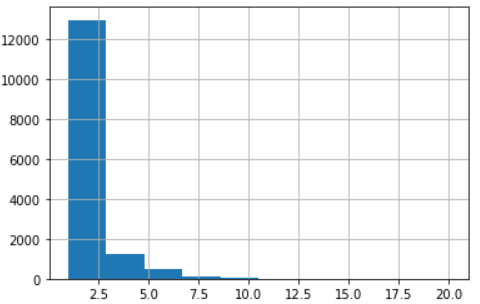
\includegraphics[scale=1]{count.png}
	\caption{Распределение количества животных в одном профиле}\label{analyse:count}
\end{figure}

Fee --- стоимость питомца. В тренировочном датасете 12663 животных отдают бесплатно и 2330 за определенную плату. Причем плата может быть как 10 малайзийских ринггитов, так и 3000 (рис. \ref{analyse:fee}). За плату чаще отдают животных, которые являются чистопородными. Например, за 3000 отдают немецкую овчарку, за 2000 английского бульдога, за 750 персидскую кошку. Но также есть беспородные животные, которых отдают за плату, например, домашнюю длинношерстную кошку за 10 малайзийских ринггитов.

\begin{figure}[H]
	\centering
	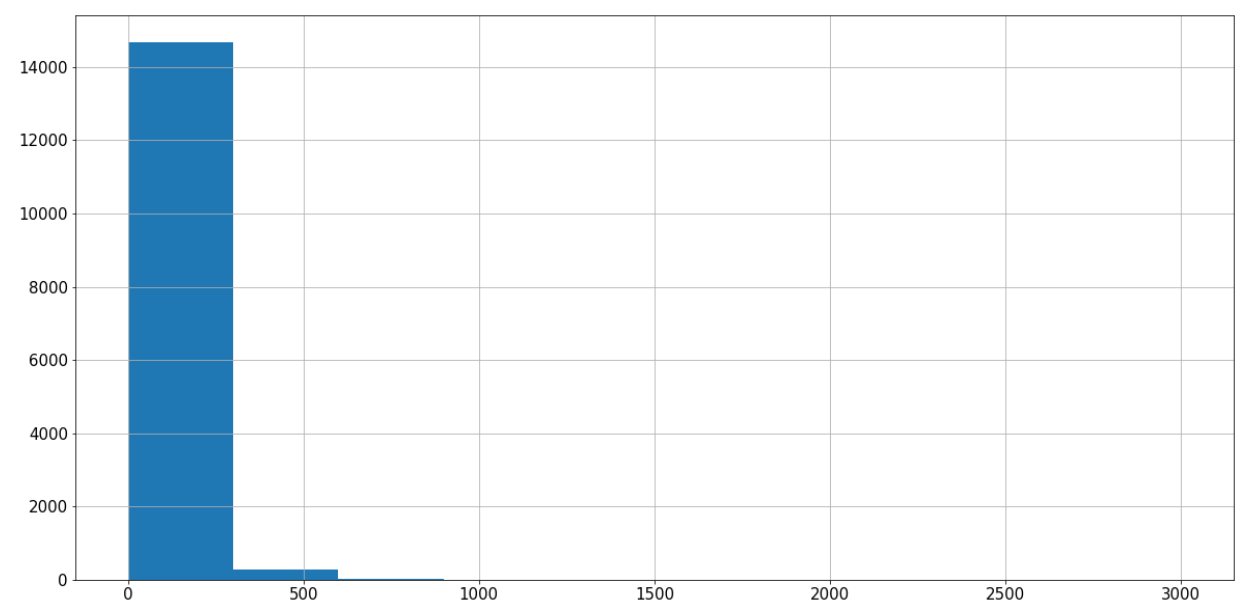
\includegraphics[scale=0.5]{fee.png}
	\caption{Гистограмма стоимости питомца}\label{analyse:fee}
\end{figure}

State --- штат в Малайзии, в котором находится питомец. Интересно, что 97\% питомцев находится в 6 штатах, а именно в Selangor, Kuala Lumpur, Pulau Pinang, Johor и Perak (рис. \ref{analyse:state}).

\begin{figure}[H]
	\centering
	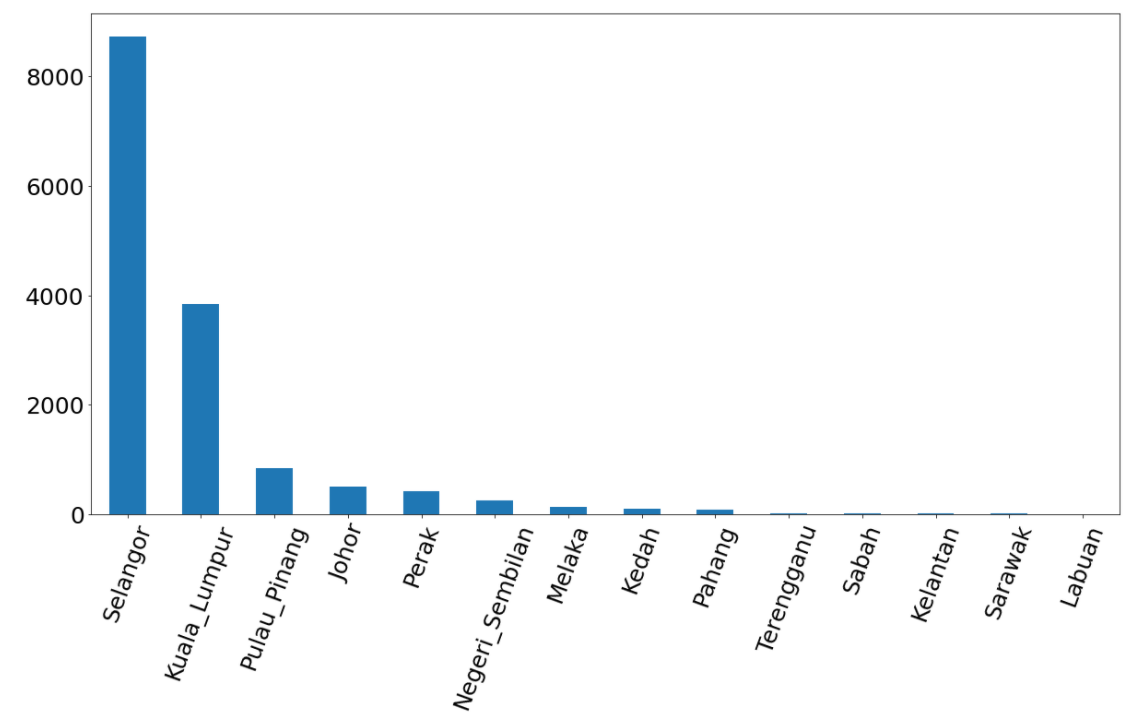
\includegraphics[scale=0.5]{state.png}
	\caption{Количество питомцев в штатах Малайзии}\label{analyse:state}
\end{figure}

RescuerID --- это идентификатор пользователя, который выкладывает профиль животного на сайт. Есть несколько людей или организаций, которые выложили достаточно много объявлений (рис. \ref{analyse:rescuer}). Наибольшее число профилей составило 459.

\begin{figure}[H]
	\centering
	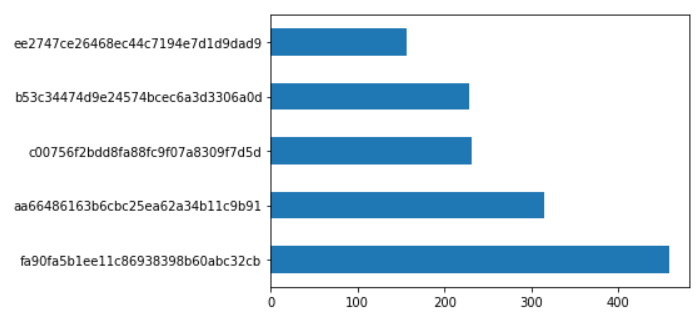
\includegraphics[scale=0.8]{rescuer.png}
	\caption{Количество профилей, которые выложили пользователи}\label{analyse:rescuer}
\end{figure}

VideoAmt и PhotoAmt содержат количество видео и фото, которые содержатся в профиле питомца.
Переменная Description хранит текстовое описание профиля. Основной используемый язык --- английский.

AdoptionSpeed --- это целевая категориальная переменная, которую необходимо предсказать. Всего имеется 5 классов:

\begin{itemize}
	\item 0 --- питомца забрали в первый же день, как профиль был создан
	\item 1 --- питомца забрали в период от 1 до 7 дней после создания профиля
	\item 2 --- питомца забрали в период от 8 до 30 дней после создания профиля
	\item 3 --- питомца забрали в период от 31 до 90 дней после создания профиля
	\item 4 --- питомец не был принят в семью после 90 дней ожидания
\end{itemize}

Для профилей, в которых несколько животных, скорость принятия в семью определяется как скорость, с которой все животные были приняты. 

AdoptionSpeed имеет сильный дисбаланс классов (рис. \ref{analyse:speed}). Количество животных, которых приняли в первый же день (0 класс), составляет 410 особей. А наибольшее число питомцев (4197 особей) находится в 4 классе. Таким образом, количество питомцев в наибольшем классе превышает количество питомцев в наименьшем классе в 10 раз.

\begin{figure}[H]
	\centering
	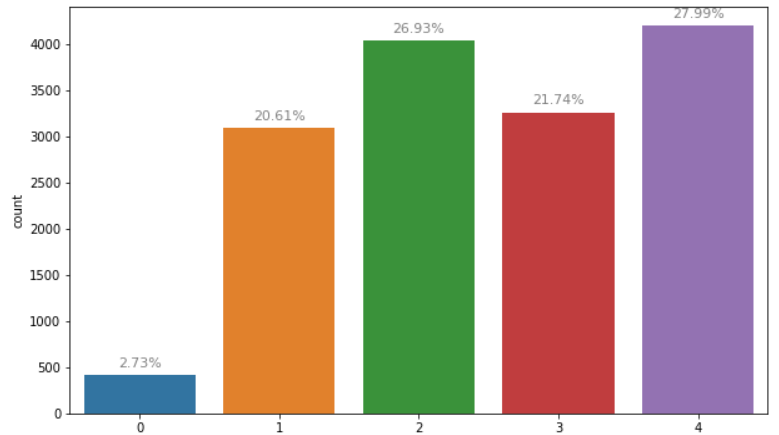
\includegraphics[scale=0.8]{speed.png}
	\caption{Количество питомцев в каждом из классов}\label{analyse:speed}
\end{figure}

Для получения корректного качества модели все признаки необходимо предобработать, а именно обработать пропущенные значение, найти и обработать выбросы, извлечь признаки из имеющихся данных, закодировать категориальные переменные, привести данные к одной шкале.

\subsection{Обработка пропущенных значений}

В датасете всего 2 переменные содержат пропущенные значения: Name и Description (рис. \ref{analyse:empty}). 

\begin{figure}[H]
	\centering
	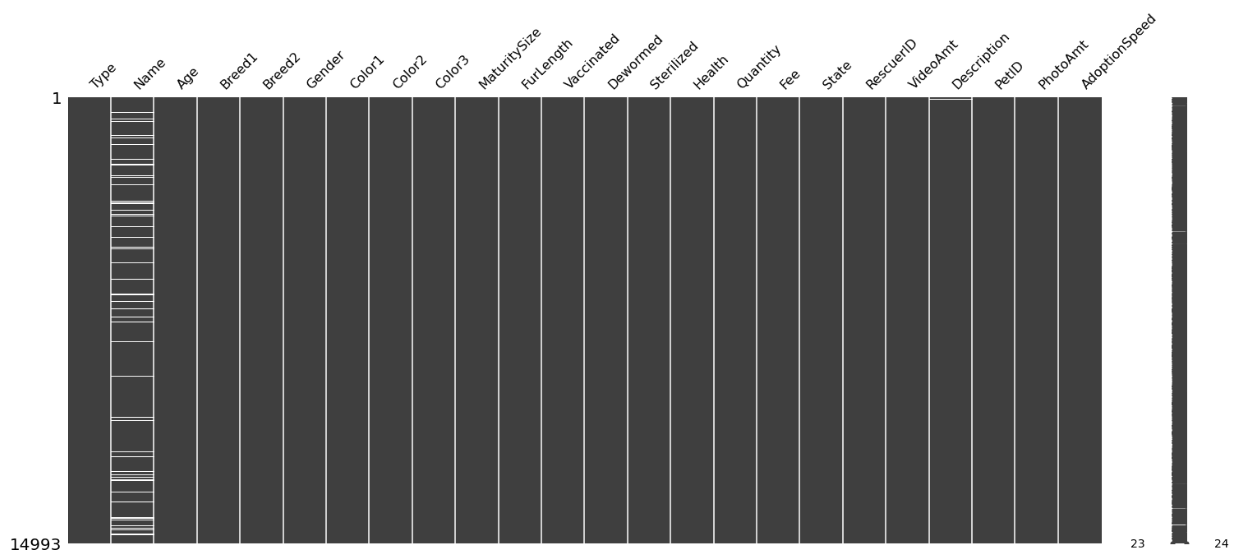
\includegraphics[scale=0.5]{empty.png}
	\caption{Пропущенные значения в данных}\label{analyse:empty}
\end{figure}

Переменная Name содержит 1257 пропусков. Это составляет 8\% от всего датасета. Переменная Description содержит 12 пропущенных значений, что составляет 0.08\% от датасета.
Пропущенные значения необходимо обрабатывать, так как не все модели способны работать с ними. Есть несколько способов борьбы с пропущенными значениями [2]:
\begin{itemize}
	\item Удалить строки, содержащие пропущенные значения
	\item Заменить пропуски выборочным значением
	\item Заменить пропуски средней/медианой/модой
	\item Заполнить случайным значением
\end{itemize}

Удаление пропущенных строк не подходит, так как при использовании данного метода значительно сокращается объём датасета и, следовательно, теряется часть информации. Третий и четвертый метод также не подходят, потому что переменные Name и Description имеют строковый тип. Поэтому остаётся только заменить пропуски выборочным значением. 
Пропуски в Name были заменены значением `No\_name', а в Description пустой строкой. В дальнейшем данные переменные будут дополнительно преобразованы.


\subsection{Детекция и обработка выбросов}

Выбросы — это наблюдения, сильно отличающиеся от остальных наблюдений в выборке. Выбросы необходимо обрабатывать, так как алгоритмы машинного обучения чувствительны к диапазону и распределению переменных [3]. Наличие выбросов в данных может привести к увеличению времени обучения, а также к снижению точности.

Для автоматического обнаружения выбросов в данных был использован метод межквартильного расстояния [4]. 

Выбросами в данном случае считаются значения, которые не попадают в диапазон $[Q1 - 1,5 \times (Q3 - Q1), Q3 - 1,5 \times (Q3 - Q1)]$, где $Q1$ и $Q3$ --- первый и третий квартиль соответственно.

Методы обработки выбросов аналогичны методам обработки пропущенных значений. 

В переменной Age достаточно много выбросов (рис. \ref{analyse:ageoutlier}). Максимальное значение возраста составило 255 месяцев. Это больше 21 года, что для кошки и собаки является достаточно большим возрастом. С помощью метода межквартильного расстояния нашли 1501 выброс и заменили их выборочным значением 27, то есть верхней границей полученного диапазона $[-13,\ 27]$.

\begin{figure}[H]
	\centering
	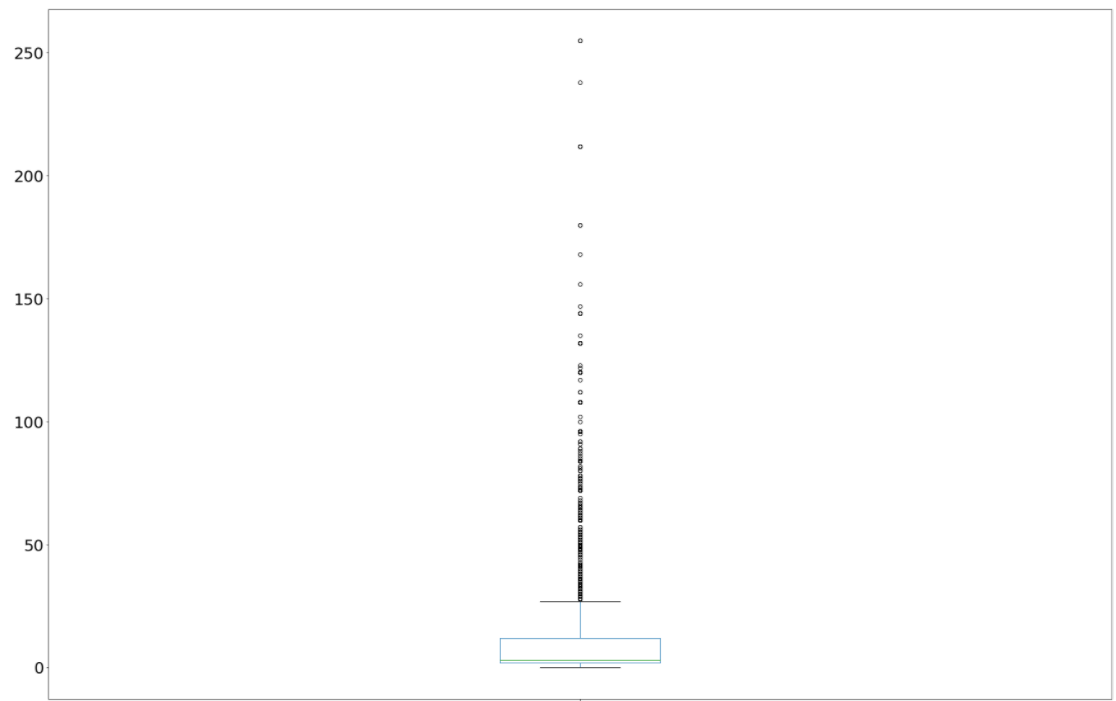
\includegraphics[scale=0.7]{ageoutlier.png}
	\caption{Выбросы в переменной Age}\label{analyse:ageoutlier}
\end{figure}

Аналогично для переменной PhotoAmt было найдено 922 выброса, которые были заменены выборочным значением 9 (рис. \ref{analyse:photooutlier}).

\begin{figure}[H]
	\centering
	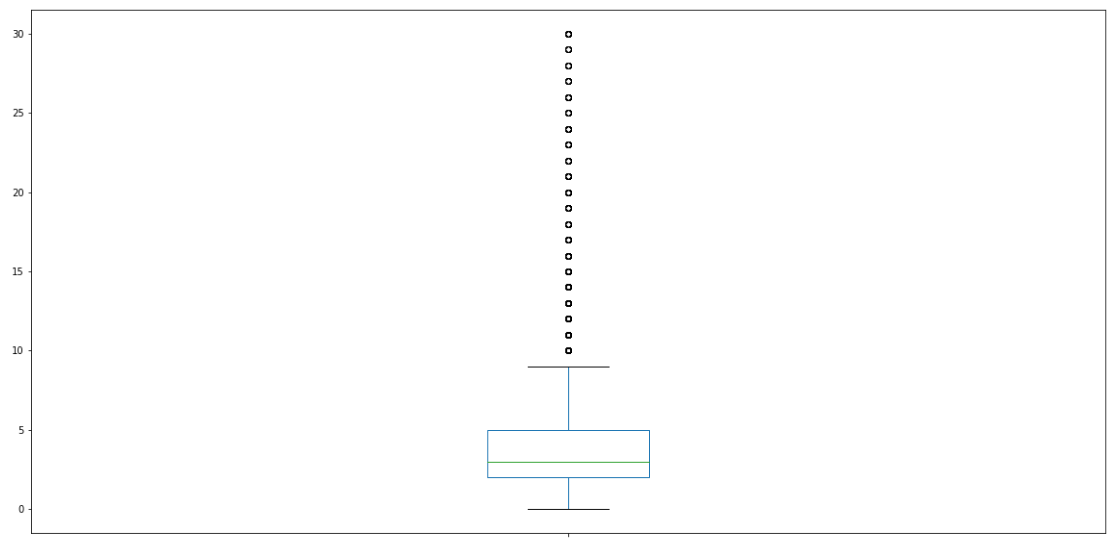
\includegraphics[scale=0.7]{photooutlier.png}
	\caption{Выбросы в переменной PhotoAmt}\label{analyse:photooutlier}
\end{figure}

Также выбросы наблюдаются в переменных Quantity и Fee. Особенностью данных переменных является то, что большая часть значений находится в 1 для Quantity и в 0 для Fee. Из-за этого на графике boxplot (рис. \ref{analyse:feeoutlier}) среднее, медиана, нижняя и верхняя границы, первый и третий квартиль сливаются в одну линию. Если заменить все выбросы верхней границей диапазона (для Quantity --- $[1,\ 1]$, для Fee --- $[0,\ 0]$), то переменная станет константной и не будет иметь значения для обучения модели. Поэтому для обработки данных переменных выбраны две стратегии:
\begin{itemize}
	\item Замена части выбросов выборочным значением
	\item Создание новой переменной, которая оценивает исходную
\end{itemize}

\begin{figure}[H]
	\centering
	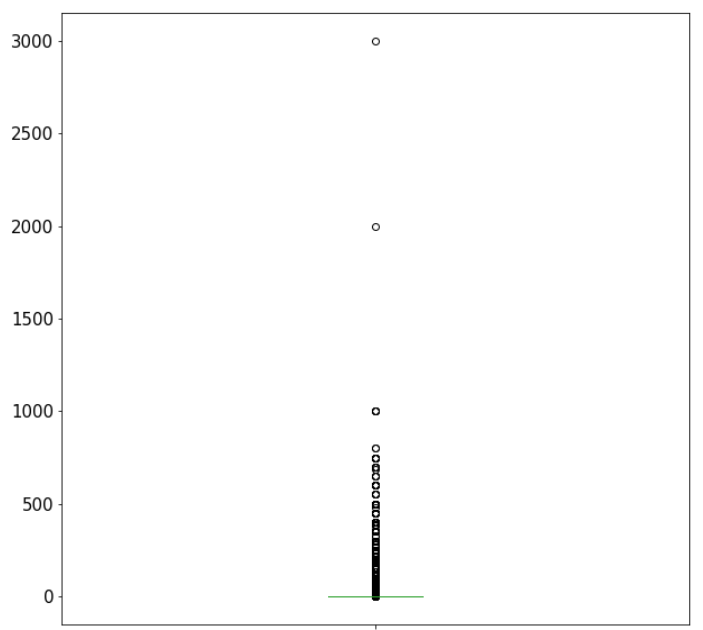
\includegraphics[scale=0.7]{feeoutlier.png}
	\caption{Выбросы в переменной Fee}\label{analyse:feeoutlier}
\end{figure}

При использовании первой стратегии в переменной Quantity заменена часть выбросов, у которых значение больше 5, значением 5, а в переменной Fee заменены значения, превышающие 500, значением 500.

При использовании второй стратегии для Quantity создана новая переменная one\_pet, которая имеет значение 1, если в профиле одно животное, и 0, если животных несколько. Аналогично для переменной Fee создана переменная Free, имеющая значение 1, если животное отдают бесплатно, иначе 0.

Таким образом, обучение будет происходить на двух датасетах, в одном из которых заменены переменные новыми, оценивающими значения, а в другом заменена часть выбросов выборочным значением.


\subsection{Создание новых признаков из имеющихся данных}

Переменная Name имеет строковый формат, и, так как модели машинного обучения не умеют работать со строковым типом, то необходимо эту переменную преобразовать. Для этого заменим признак Name новой переменной No\_name, которая будет обозначать, есть ли у животного реальное имя. На этапе обработки пропущенных значений всем значениям равным NaN было поставлено значение `No\_name'. Также в поле Name есть значения, которые обозначают отсутствие имени. Например, ``unnamed'', ``nameless'', ``no name yet''. Ещё есть очень короткие имена, состоящие из 1–3 символов и не имеющие смысла. Все эти значения также были заменены на `No\_name'. Затем новой переменной No\_name присваиваем значение 1, если в Name стоит значение `No\_name', иначе ставим 0. Таким образом, вместо строковой переменной Name получили булеву переменную No\_name (рис. \ref{analyse:hasname}), которую и будем использовать в обучении.

\begin{figure}[H]
	\centering
	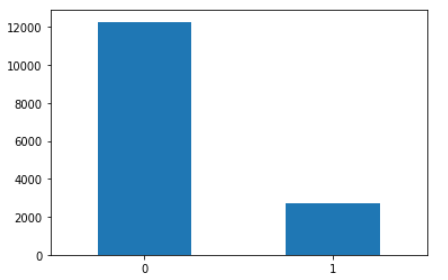
\includegraphics[scale=1]{hasname.png}
	\caption{Число питомцев, имеющих имя и не имеющих}\label{analyse:hasname}
\end{figure}

Из переменных Breed1 и Breed2 была создана новая переменная Pure\_breed (рис. \ref{analyse:purebreed}), обозначающая, является ли животное породным или беспородным. Породным считалось животное, которое в Breed2 имеет значение 0 (то есть нет расшифровки в словаре) и в Breed1 не имеет значения `Mixed\_Breed', `Domestic\_Long\_Hair', `Domestic\_Medium\_Hair' или \\ `Domestic\_Short\_Hair', так как данные виды не считаются породистыми.

\begin{figure}[H]
	\centering
	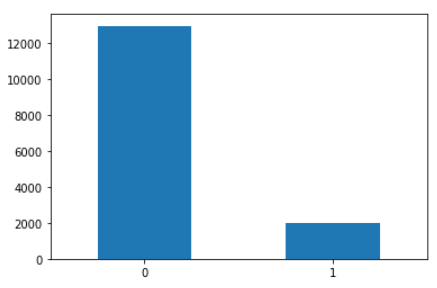
\includegraphics[scale=1]{purebreed.png}
	\caption{Число породных и беспородных питомцев}\label{analyse:purebreed}
\end{figure}

Переменная RescuerID содержит идентификатор людей или организаций, которые создают профиль питомца на сайте, а также отдают его. Есть идентификаторы, которые создали достаточно много профилей (рис. \ref{analyse:toprescuer}). 

\begin{figure}[H]
	\centering
	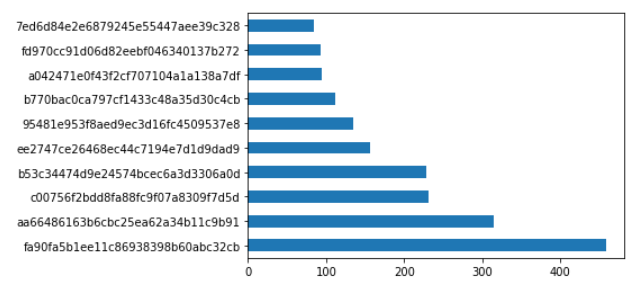
\includegraphics[scale=1]{toprescuer.png}
	\caption{Топ-10 пользователей, создавших наибольшее число профилей}\label{analyse:toprescuer}
\end{figure}

Самое наибольшее --- 459 профилей. Но так как данная переменная строкового типа, а всего уникальных значений 5415, то невозможно считать её категориальной, так как очень сильно расширится пространство признаков при использовании OneHotEncoding, что может негативно сказаться на времени обучения и качестве модели. Поэтому была создана новая переменная RankRescuer. Это переменная обозначает рейтинг пользователей, кто на каком месте по количеству объявлений. То есть пользователь с 459 объявлениями на 1 месте, с 315 --- на 2 и так далее. Если у кого-то совпадает количество объявлений, то они делят одно место. Таким образом, в RankRescuer получилось 61 значение.

Из переменной VideoAmt (количество видео) была создана новая переменная has\_video, которая обозначает наличие видео в профиле. Это было сделано из-за того, что VideoAmt в основном принимает значение 0, а остальные значения считаются выбросами (рис. \ref{analyse:videooutlier}).

\begin{figure}[H]
	\centering
	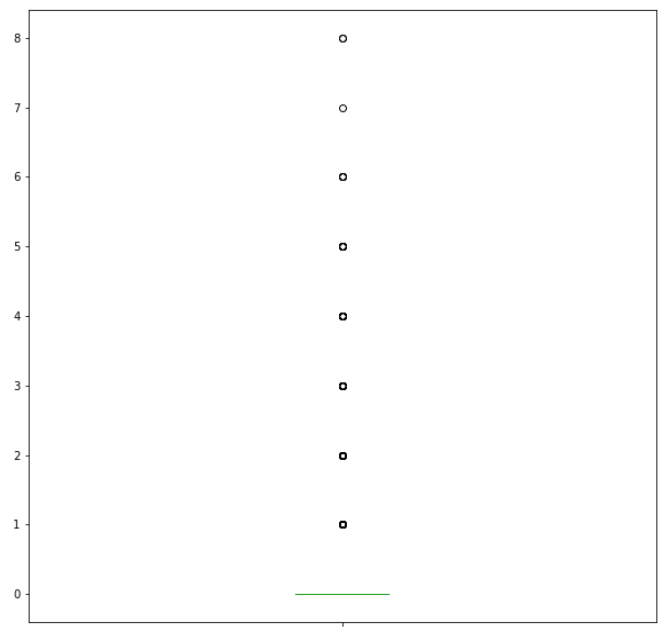
\includegraphics[scale=0.6]{videooutlier.png}
	\caption{Boxplot для VideoAmt}\label{analyse:videooutlier}
\end{figure}

В переменной Description находится описание питомцев. Для каждого описания создатели задачи выполнили анализ эмоциональной окраски текста с помощью Google’s Natural Language API и записали результаты в файлы формата JSON. 

Из данных из этих файлов были созданы новые переменные lang, magnitude и score. В переменной lang хранится язык, на котором написаны описания (рис.\ref{analyse:lang}). Модель Google’s Natural Language распознала английский (en), китайский упрощенный (zh), китайский традиционный (zh-Hant) и немецкий (de). Также есть часть наблюдений, где модель не смогла распознать, на каком языке написан текст. Этим наблюдениям присвоено значение `no' в переменной lang. Наблюдений на немецком языке всего 2 штуки, поэтому они были удалены из датасета, чтоб не увеличивать количество категорий. С этой же целью китайский традиционный и китайский упрощенный были объеденены в один язык. 

\begin{figure}[H]
	\centering
	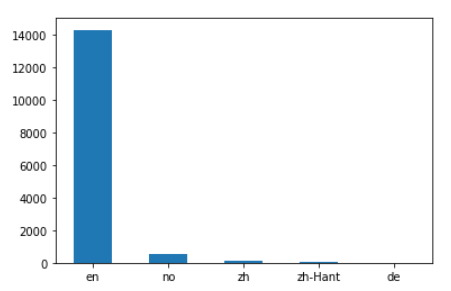
\includegraphics[scale=1.2]{lang.png}
	\caption{Значения переменной lang}\label{analyse:lang}
\end{figure}

Score --- это переменная со значениями из диапазона $[-1,\ 1]$. Отрицательное значение указывает на негативную окраску, положительное --- на положительную. Чем ближе это значение к нулю, тем более текст нейтрален. Magnitude указывает, насколько эмоционален текст [5]. 


\subsection{Кодирование категориальных переменных}

\subsection{Шкалирование переменных}

%=======================
\newpage
\section{Используемая метрика}

%=======================
\newpage
\section{Использованные модели}

\subsection{Baseline}

\subsection{Дерево решений}

\subsection{Логистическая регрессия}

\subsection{Случайный лес}

\subsection{Градиентный бустинг}

%=======================
\newpage
\section{Классификация только с использованием текстовых признаков}

\subsection{Предобработка текстов и выделение признаков}

\subsection{Обучение модели}

\subsection{Полученные результаты}

%=======================
\newpage
\section{Выбор датасета, модели и тестирование на Kaggle}


%=======================
\newpage
\addcontentsline{toc}{section}{Заключение}
\section*{Заключение}

Заключение должно содержать информацию о проделанной работе и полученных результатах.

При написании текста работы следует иметь в виду, что её цель состоит в том, чтобы продемонстрировать квалификацию автора. Поэтому следует избегать общих и, тем более, тривиальных или нравоучительных высказываний. Мотивация выполняемой работы не должна носить слишком конкретный характер. Во время выступления на защите желательно избегать упоминаний об особенностях стандартных компонентов пользовательского интерфейса программ (<<нажимаем на правую кнопку>>, <<перетаскиваем фрагмент мышью>> и т.\,д.). Не следует комментировать задаваемые после защиты вопросы. Ответы на вопросы должны быть краткими.



%=======================
\newpage

\addcontentsline{toc}{section}{Литература}
\renewcommand{\refname}{\centering \textbf{Литература}}

\begin{thebibliography}{0}
\bibitem{stud:b0}
Рекомендации по оформлению
и представлению курсовых
и выпускных квалификационных работ
студентов института математики,
механики и компьютерных наук.~--
Ростов н/Д, 2020.

\bibitem{stud:b1}
Жуков М.\,Ю., Ширяева Е.\,В.
\LaTeXe: искусство набора и вёрстки текстов с~формулами.~-- Ростов н/Д : Изд-во ЮФУ, 2009.
\end{thebibliography}

%=======================
\newpage

\addcontentsline{toc}{section}{Приложение}
\section*{Приложение}



\end{document}
% ----------------------------------------------------------------


\lstset{ %
language=C++,                 % выбор языка для подсветки (здесь это С++)
basicstyle=\small\sffamily, % размер и начертание шрифта для подсветки кода
numbers=left,               % где поставить нумерацию строк (слева\справа)
numberstyle=\tiny,           % размер шрифта для номеров строк
stepnumber=1,                   % размер шага между двумя номерами строк
numbersep=5pt,                % как далеко отстоят номера строк от подсвечиваемого кода
backgroundcolor=\color{white}, % цвет фона подсветки - используем \usepackage{color}
showspaces=false,            % показывать или нет пробелы специальными отступами
showstringspaces=false,      % показывать или нет пробелы в строках
showtabs=false,             % показывать или нет табуляцию в строках
frame=single,              % рисовать рамку вокруг кода
tabsize=2,                 % размер табуляции по умолчанию равен 2 пробелам
captionpos=t,              % позиция заголовка вверху [t] или внизу [b]
breaklines=true,           % автоматически переносить строки (да\нет)
breakatwhitespace=false, % переносить строки только если есть пробел
escapeinside={\%*}{*)}   % если нужно добавить комментарии в коде
extendedchars=true,
commentstyle=\color{mygreen},    % comment style
stringstyle=\bf,
commentstyle=\ttfamily\itshape,
keepspaces=true % пробелы между русскими буквами
aboveskip=3mm,
belowskip=3mm

}


\renewcommand\NAT@bibsetnum[1]{\settowidth\labelwidth{\@biblabel{#1}}%
   \setlength{\leftmargin}{\bibindent}\addtolength{\leftmargin}{\dimexpr\labelwidth+\labelsep\relax}%
   \setlength{\itemindent}{-\bibindent+\fivecharsapprox}%
   \setlength{\listparindent}{\itemindent}
\setlength{\itemsep}{\bibsep}\setlength{\parsep}{\z@}%
   \ifNAT@openbib
     \addtolength{\leftmargin}{\bibindent}%
     \setlength{\itemindent}{-\bibindent}%
     \setlength{\listparindent}{\itemindent}%
     \setlength{\parsep}{0pt}%
   \fi
}
\renewcommand{\thesection}{\arabic{section}.}
\renewcommand{\thesubsection}{\arabic{section}.\arabic{subsection}.}
